%==========================================================
\section{Consolidação dos modelos}\label{sec:consolidacao}

A consolidação junta os modelos individuais para mostrar a estrutura comum do trabalho, em vez de casos isolados~\cite[cap.~9]{beyer1998}. Foi aplicada às duas sessões (A0 e U0), que representam as duas populações do problema: quem planeia a viagem e quem a planeia profissionalmente.

%----------------------------------------------------------
\subsection{Fluxo consolidado}\label{sec:fluxo-cons}

\paragraph{Método.} Seguiram-se os passos do livro~\cite[pp.~163--170]{beyer1998}:
\begin{enumerate}
  \item listar as responsabilidades de cada pessoa, grupo e lugar nos fluxos individuais;
  \item agrupar as responsabilidades em \textbf{papéis}, cada um com uma intenção principal; só é papel o que se poderia atribuir a uma pessoa contratada para isso;
  \item juntar papéis semelhantes vindos de modelos diferentes e dar-lhes um nome simples;
  \item redesenhar as comunicações e os artefactos entre papéis, com nomes abstratos;
  \item copiar os \textit{breakdowns} dos modelos individuais;
  \item colorir cada papel pela população que o desempenha (viajante, agente ou não entrevistado).
\end{enumerate}

\begin{figure}[!htbp]
\centering
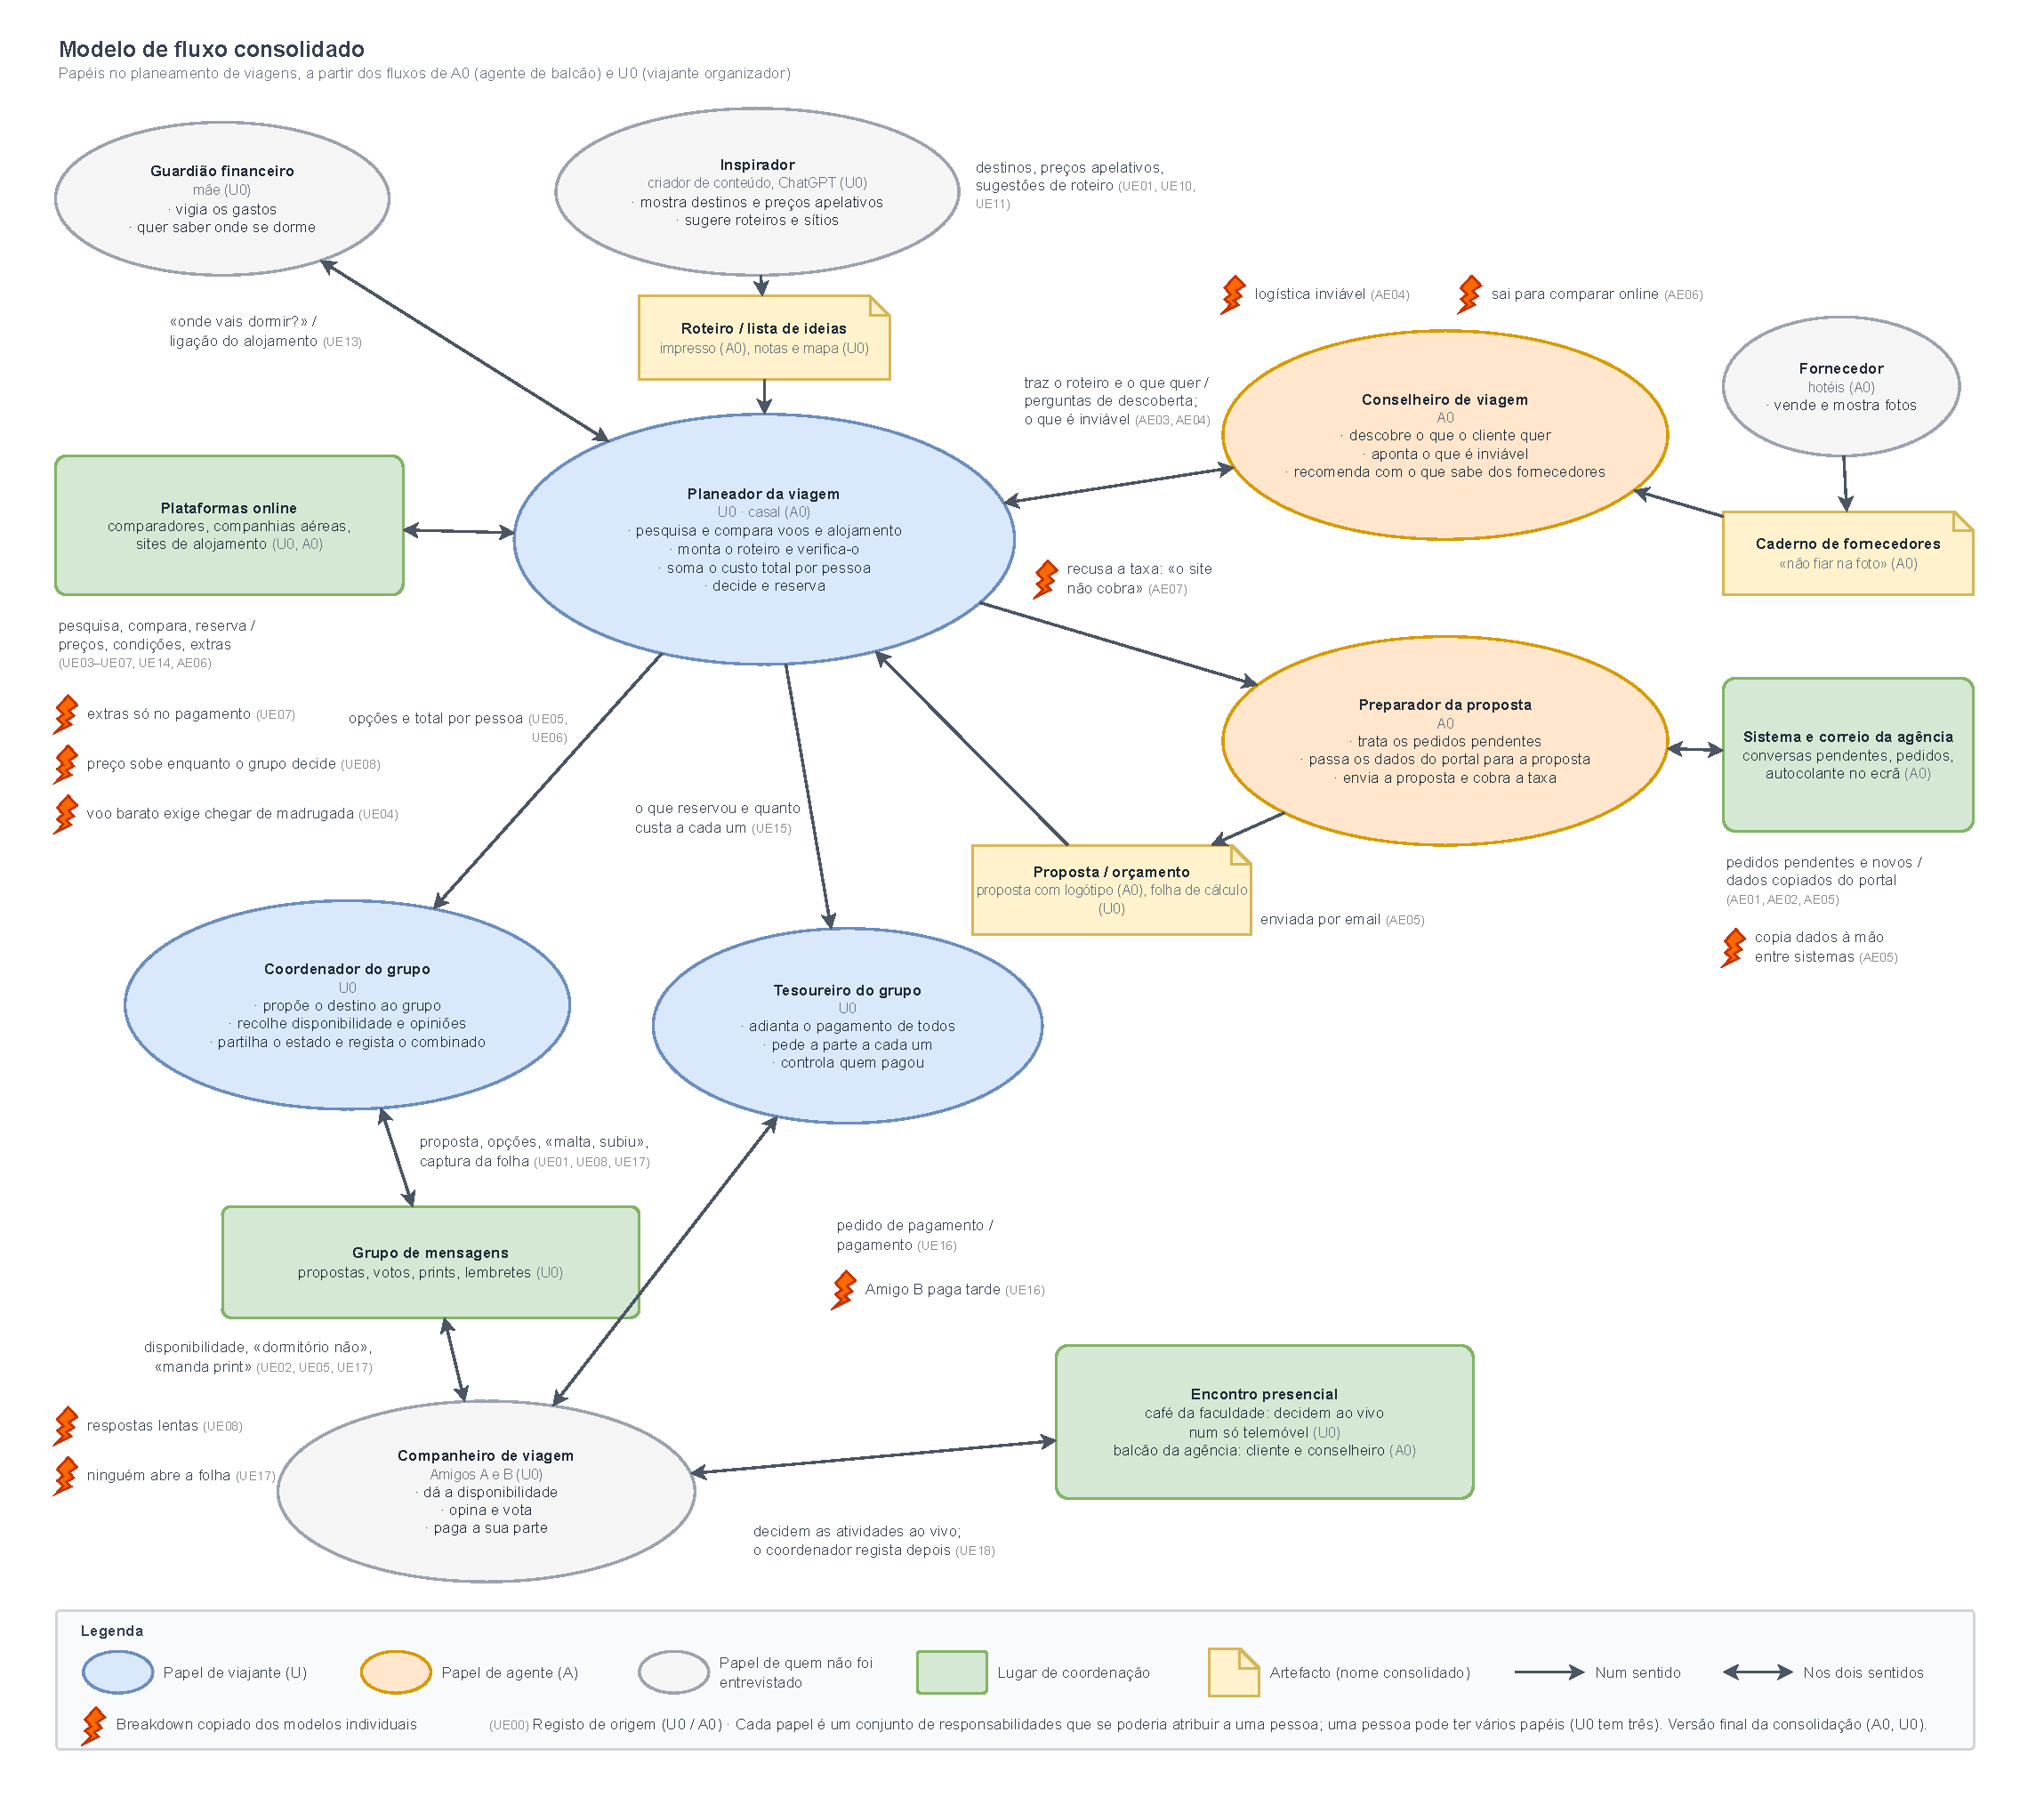
\includegraphics[width=\textwidth]{flow_models/consolidado/FluxoConsolidado.drawio.pdf}
\caption{Modelo de fluxo consolidado (A0 e U0).}
\label{fig:fluxo-cons}
\end{figure}

\paragraph{Papéis.} A Tabela~\ref{tab:papeis-cons} mostra os nove papéis identificados e quem os desempenha.

\begin{table}[!htbp]
\centering\small
\begin{tabularx}{\textwidth}{@{}p{3.4cm}Lp{2.8cm}@{}}
\toprule
\textbf{Papel} & \textbf{Responsabilidades} & \textbf{Desempenhado por} \\
\midrule
\rowcolor{blue!6} Planeador da viagem & Pesquisa e compara voos e alojamento; monta o roteiro e verifica-o; soma o custo total por pessoa; decide e reserva. & U0; casal (A0) \\
\rowcolor{blue!6} Coordenador do grupo & Propõe o destino; recolhe disponibilidade e opiniões; partilha o estado e regista o combinado. & U0 \\
\rowcolor{blue!6} Tesoureiro do grupo & Adianta o pagamento de todos; pede a parte a cada um; controla quem pagou. & U0 \\
\rowcolor{orange!10} Conselheiro de viagem & Descobre o que o cliente quer; aponta o que é inviável; recomenda com o que sabe dos fornecedores. & A0 \\
\rowcolor{orange!10} Preparador da proposta & Trata os pedidos pendentes; passa os dados do portal para a proposta; envia-a e cobra a taxa. & A0 \\
Inspirador & Mostra destinos e preços apelativos; sugere roteiros e sítios. & Criador de conteúdo, ChatGPT \\
Guardião financeiro & Vigia os gastos; quer saber onde se dorme. & Mãe de U0 \\
Companheiro de viagem & Dá a disponibilidade; opina e vota; paga a sua parte. & Amigos A e B \\
Fornecedor & Vende e mostra fotos. & Hotéis \\
\bottomrule
\end{tabularx}
\caption{Papéis do fluxo consolidado. Azul: viajante; laranja: agente; branco: não entrevistado.}
\label{tab:papeis-cons}
\end{table}

\paragraph{Lugares e artefactos consolidados.} \textbf{Plataformas online} junta comparadores, companhias aéreas e sites de alojamento (U0, A0). \textbf{Encontro presencial} junta o café da faculdade (U0) e o balcão da agência (A0). \textbf{Roteiro / lista de ideias} junta o roteiro impresso do casal (A0) com as notas e a lista no mapa de U0. \textbf{Proposta / orçamento} junta a proposta com logótipo (A0) com a folha de cálculo de U0.

\paragraph{O que o fluxo consolidado mostra.}
\begin{itemize}
  \item \textbf{Uma só pessoa acumula três papéis.} U0 é planeador, coordenador e tesoureiro. Não há nenhuma ferramenta que apoie os três ao mesmo tempo; cada papel tem o seu sítio (folha, grupo de mensagens, pedido de pagamento).
  \item \textbf{O agente desempenha papéis que o viajante faz sozinho.} O conselheiro (descobrir o que se quer, apontar o que é inviável) faz o que U0 faz ao verificar no mapa as sugestões da IA. É este o espaço que o \projeto{} quer ocupar.
  \item \textbf{A proposta é o artefacto central nos dois mundos.} Para o agente é o documento com logótipo; para o viajante é a folha de cálculo. Nos dois casos é montada à mão a partir de dados copiados de outros sistemas.
  \item \textbf{Os \textit{breakdowns} concentram-se nas passagens entre papéis}: entre plataformas e planeador (custos escondidos, preços que sobem), entre coordenador e companheiros (respostas lentas, folha que ninguém abre) e entre tesoureiro e companheiros (pagamentos em atraso).
\end{itemize}

%----------------------------------------------------------
\subsection{Cultural consolidado}\label{sec:cultural-cons}

\paragraph{Método.} Seguiram-se os passos do livro~\cite[pp.~190--198]{beyer1998}:
\begin{enumerate}
  \item catalogar os influenciadores dos modelos individuais;
  \item agrupar os que condicionam o trabalho da mesma forma;
  \item recolher as influências e agrupá-las pelo par de influenciadores entre os quais vão;
  \item eliminar duplicados e escolher uma redação que mostre o tom emocional da influência;
  \item desenhar o modelo final e copiar os \textit{breakdowns}.
\end{enumerate}

\begin{figure}[!htbp]
\centering
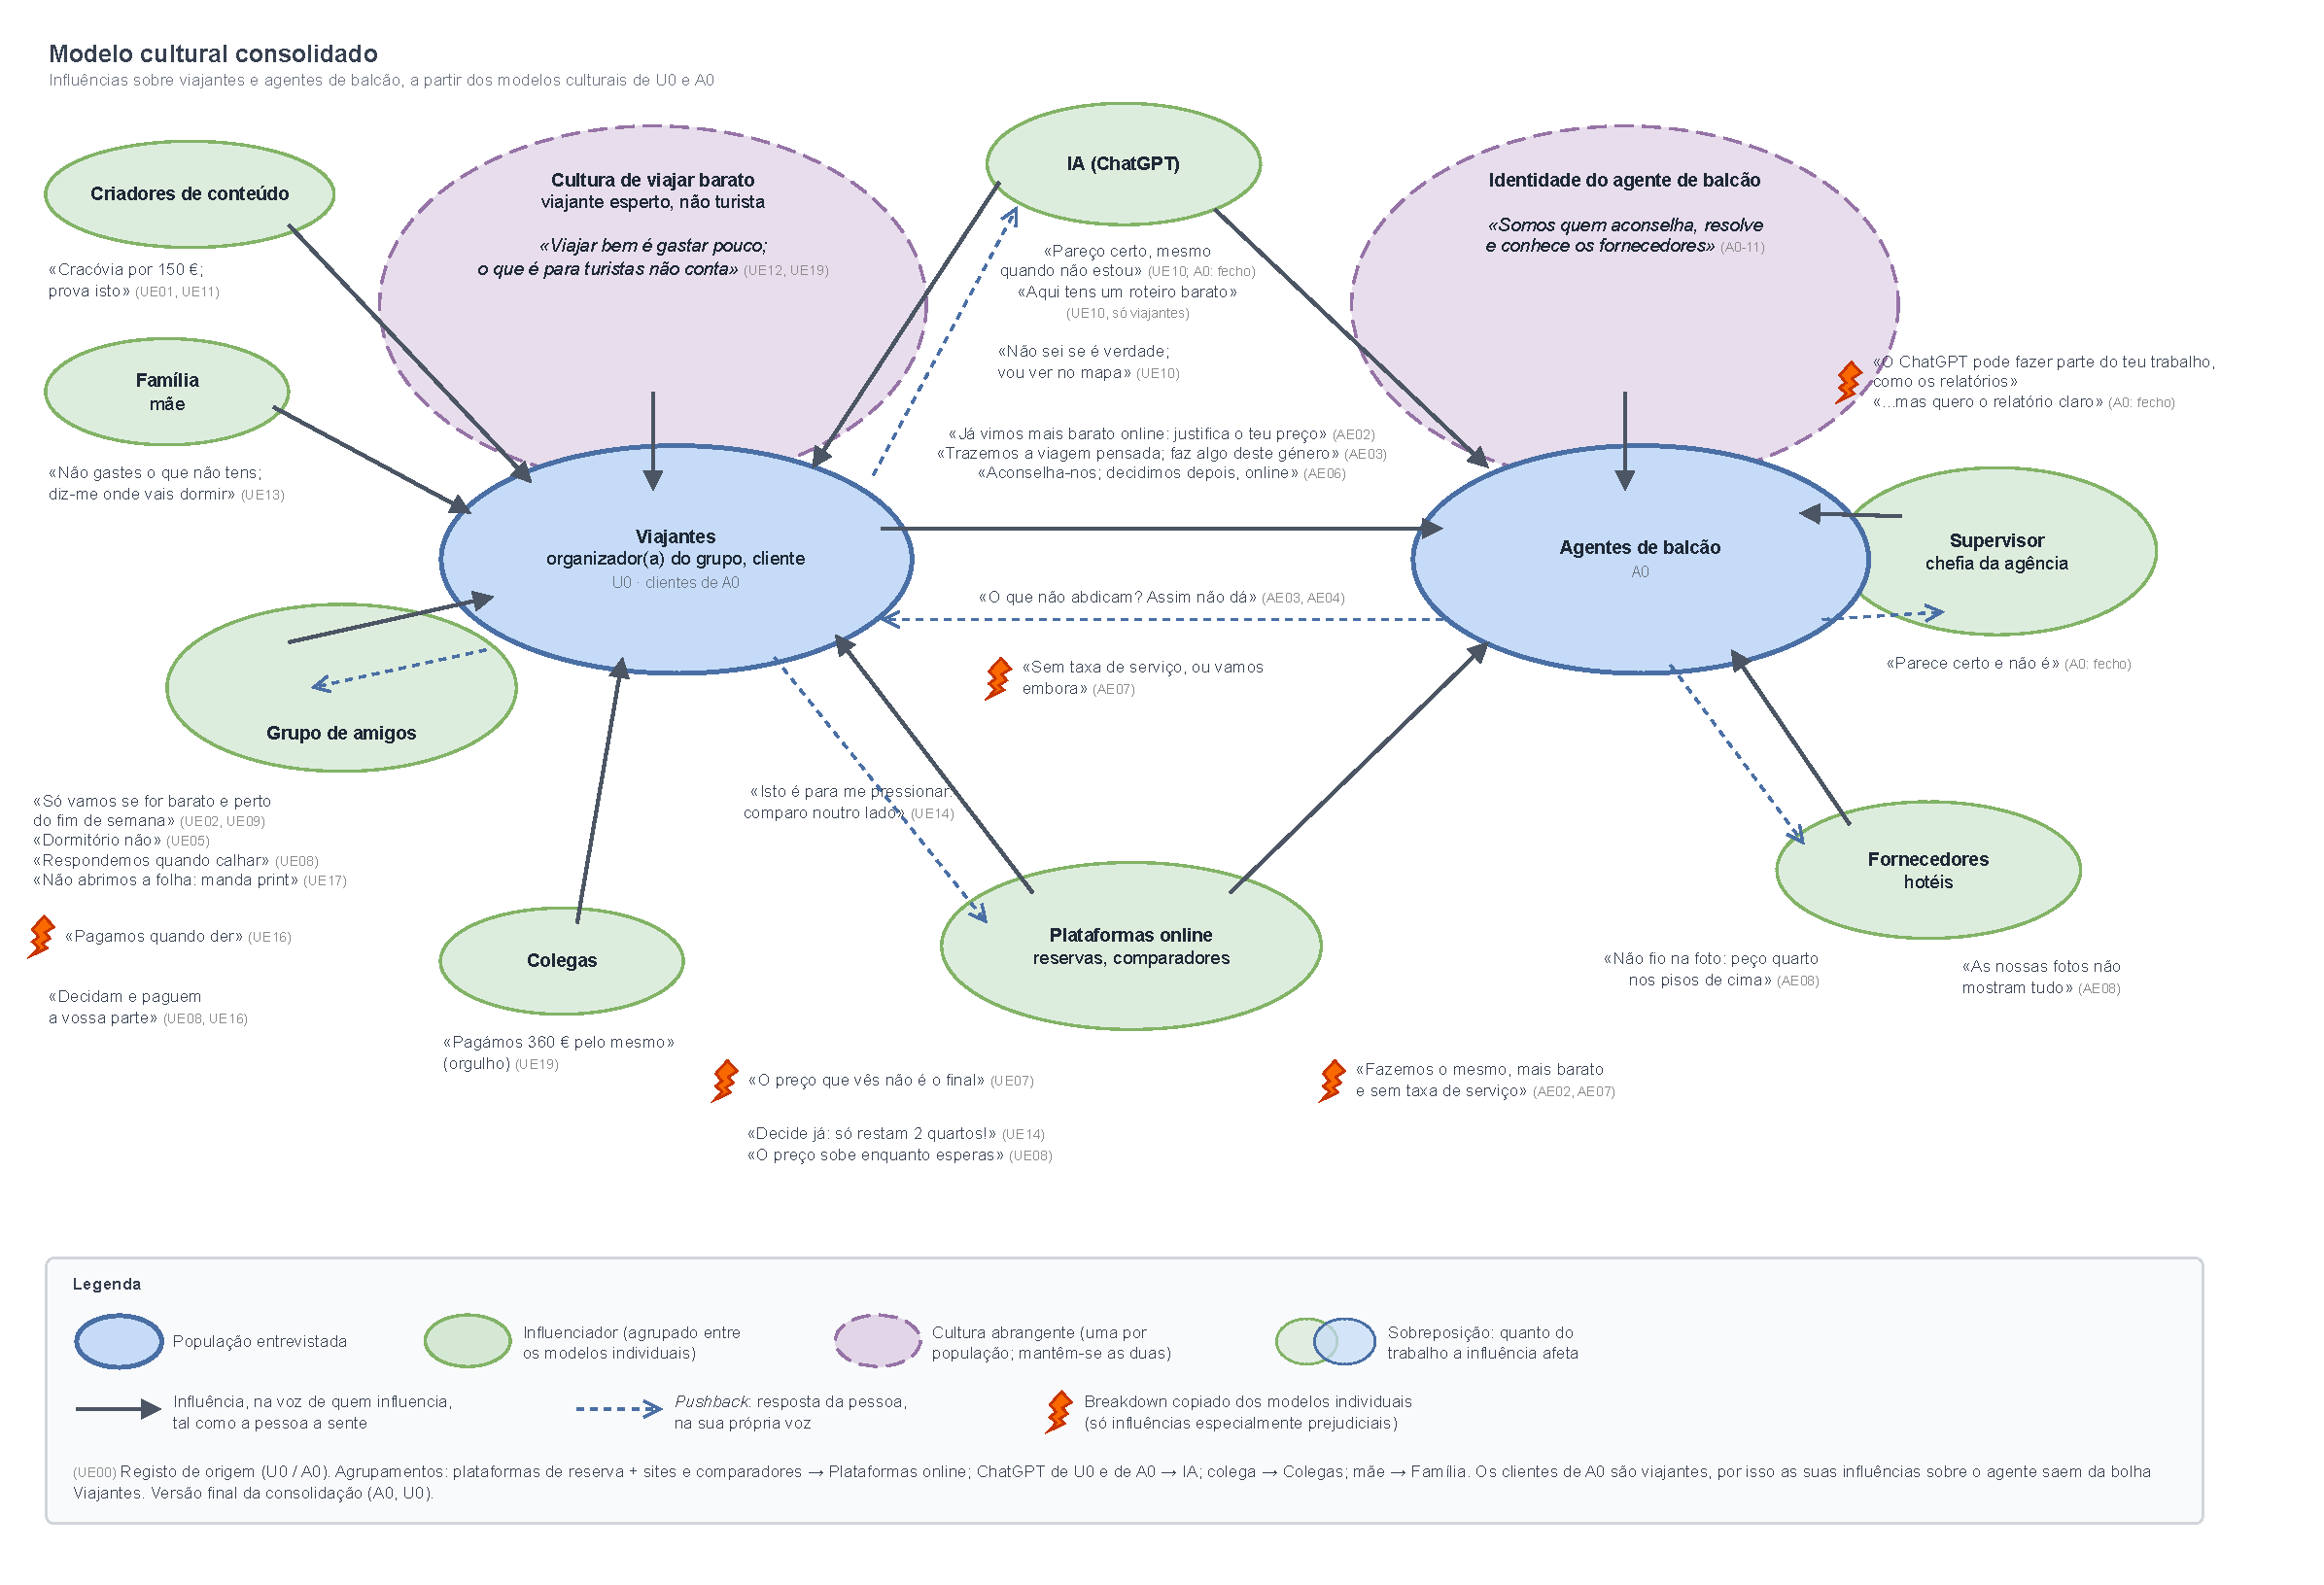
\includegraphics[width=\textwidth]{cultural_models/consolidado/CulturalConsolidado.drawio.pdf}
\caption{Modelo cultural consolidado (A0 e U0).}
\label{fig:cultural-cons}
\end{figure}

\begin{table}[!htbp]
\centering\small
\begin{tabularx}{\textwidth}{@{}p{4.4cm}p{3.4cm}L@{}}
\toprule
\textbf{Nos modelos individuais} & \textbf{No modelo consolidado} & \textbf{Porquê} \\
\midrule
Plataformas de reserva (U0); sites e comparadores (A0) & Plataformas online & Pressionam da mesma forma: preço, urgência, ausência de taxa. \\
ChatGPT (U0); ChatGPT (A0) & IA (ChatGPT) & A mesma ferramenta, sentida com a mesma desconfiança. \\
Clientes (A0) & Viajantes & Os clientes de A0 são viajantes; as suas influências saem da bolha Viajantes. \\
Colega (U0) & Colegas & Referência de preço entre pares. \\
Mãe (U0) & Família & Financia e vigia. \\
Amigos A e B (U0) & Grupo de amigos & -- \\
Supervisor, fornecedores (A0) & Supervisor, fornecedores & -- \\
\bottomrule
\end{tabularx}
\caption{Agrupamento dos influenciadores na consolidação cultural.}
\label{tab:agrup-cult}
\end{table}

\paragraph{O que o cultural consolidado mostra.}
\begin{itemize}
  \item \textbf{Duas culturas diferentes, mantidas lado a lado.} Os viajantes vivem na cultura de viajar barato; os agentes na identidade de quem aconselha e conhece os fornecedores. O livro recomenda manter culturas diferentes quando a consolidação as revela.
  \item \textbf{As duas populações influenciam-se.} Os viajantes pressionam o agente com os preços online e recusam a taxa; o agente responde apontando o que é inviável.
  \item \textbf{As plataformas online pesam sobre as duas populações}: sobre o viajante como adversárias (custos escondidos, falsa escassez) e sobre o agente como concorrentes («fazemos o mesmo, sem taxa»).
  \item \textbf{A desconfiança da IA é comum.} «Pareço certo, mesmo quando não estou» aparece nos dois modelos: o viajante verifica no mapa, o agente teme ser substituído por algo que erra.
\end{itemize}

%----------------------------------------------------------
\subsection{Restantes modelos consolidados}\label{sec:outros-cons}

\pendente{Gonçalo (sequência e artefacto) e Zé Pedro (físico)}{%
O enunciado pede pelo menos o fluxo, a sequência e mais um modelo consolidado. Incluir aqui a sequência consolidada (obrigatória) e, se houver, o artefacto e o físico consolidados, com o mesmo formato: método, figura e o que o modelo mostra.}

%----------------------------------------------------------
\subsection{Implicações para o design}\label{sec:implicacoes}

A Tabela~\ref{tab:implicacoes} liga os principais \textit{breakdowns} dos modelos de fluxo e culturais às hipóteses de produto do \textit{backlog} da equipa (Apêndice~\ref{anx:hipoteses}). Esta ligação garante que cada hipótese assenta em dados de campo e não em suposições.

\begin{table}[!htbp]
\centering\small
\begin{tabularx}{\textwidth}{@{}Lp{2.1cm}Lp{1.6cm}@{}}
\toprule
\textbf{Breakdown ou influência} & \textbf{Origem} & \textbf{Implicação para o design} & \textbf{Hipótese} \\
\midrule
Bagagem e extras só aparecem no pagamento & UE07 & Mostrar o custo total real por pessoa antes de qualquer reserva. & US-02, RF-03 \\
Voo barato exige chegar de madrugada sem transporte & UE04 & Incluir custo e tempo de chegada ao aeroporto nas comparações. & US-03, RF-04 \\
Preço sobe enquanto o grupo decide; respostas lentas & UE08 & Avisar de variações de preço e dar um prazo de decisão ao grupo. & US-05, RF-06 \\
Ninguém abre a folha; «manda print» & UE17 & Partilhar a proposta num link legível sem conta, com votação. & US-04, RF-05 \\
Organizador adianta o dinheiro; amigo paga tarde & UE15, UE16 & Dividir despesas e acompanhar quem já pagou. & US-06, RF-07 \\
«Só restam 2 quartos!» sentido como manipulação & UE14 & Não usar urgência nem escassez falsas. & RNF-02 \\
IA «parece certa e não é» & UE10; fecho A0 & Explicar porque recomenda e de onde vêm os preços. & US-09, RF-10 \\
Roteiro do cliente com logística inviável & AE04 & Validar a logística (distâncias, horários) antes de propor. & RF-02 \\
Supervisor vê a IA como substituto do agente & Fecho A0 & Permitir revisão humana da proposta por um agente. & US-13, RF-13 \\
Agente copia dados à mão entre sistemas & AE05 & Gerar a proposta diretamente a partir das opções escolhidas. & RF-02 \\
\bottomrule
\end{tabularx}
\caption{Dos \textit{breakdowns} às hipóteses de produto.}
\label{tab:implicacoes}
\end{table}
